\documentclass[1p]{elsarticle_modified}
%\bibliographystyle{elsarticle-num}

%\usepackage[colorlinks]{hyperref}
%\usepackage{abbrmath_seonhwa} %\Abb, \Ascr, \Acal ,\Abf, \Afrak
\usepackage{amsfonts}
\usepackage{amssymb}
\usepackage{amsmath}
\usepackage{amsthm}
\usepackage{scalefnt}
\usepackage{amsbsy}
\usepackage{kotex}
\usepackage{caption}
\usepackage{subfig}
\usepackage{color}
\usepackage{graphicx}
\usepackage{xcolor} %% white, black, red, green, blue, cyan, magenta, yellow
\usepackage{float}
\usepackage{setspace}
\usepackage{hyperref}

\usepackage{tikz}
\usetikzlibrary{arrows}

\usepackage{multirow}
\usepackage{array} % fixed length table
\usepackage{hhline}

%%%%%%%%%%%%%%%%%%%%%
\makeatletter
\renewcommand*\env@matrix[1][\arraystretch]{%
	\edef\arraystretch{#1}%
	\hskip -\arraycolsep
	\let\@ifnextchar\new@ifnextchar
	\array{*\c@MaxMatrixCols c}}
\makeatother %https://tex.stackexchange.com/questions/14071/how-can-i-increase-the-line-spacing-in-a-matrix
%%%%%%%%%%%%%%%

\usepackage[normalem]{ulem}

\newcommand{\msout}[1]{\ifmmode\text{\sout{\ensuremath{#1}}}\else\sout{#1}\fi}
%SOURCE: \msout is \stkout macro in https://tex.stackexchange.com/questions/20609/strikeout-in-math-mode

\newcommand{\cancel}[1]{
	\ifmmode
	{\color{red}\msout{#1}}
	\else
	{\color{red}\sout{#1}}
	\fi
}

\newcommand{\add}[1]{
	{\color{blue}\uwave{#1}}
}

\newcommand{\replace}[2]{
	\ifmmode
	{\color{red}\msout{#1}}{\color{blue}\uwave{#2}}
	\else
	{\color{red}\sout{#1}}{\color{blue}\uwave{#2}}
	\fi
}

\newcommand{\Sol}{\mathcal{S}} %segment
\newcommand{\D}{D} %diagram
\newcommand{\A}{\mathcal{A}} %arc


%%%%%%%%%%%%%%%%%%%%%%%%%%%%%5 test

\def\sl{\operatorname{\textup{SL}}(2,\Cbb)}
\def\psl{\operatorname{\textup{PSL}}(2,\Cbb)}
\def\quan{\mkern 1mu \triangleright \mkern 1mu}

\theoremstyle{definition}
\newtheorem{thm}{Theorem}[section]
\newtheorem{prop}[thm]{Proposition}
\newtheorem{lem}[thm]{Lemma}
\newtheorem{ques}[thm]{Question}
\newtheorem{cor}[thm]{Corollary}
\newtheorem{defn}[thm]{Definition}
\newtheorem{exam}[thm]{Example}
\newtheorem{rmk}[thm]{Remark}
\newtheorem{alg}[thm]{Algorithm}

\newcommand{\I}{\sqrt{-1}}
\begin{document}

%\begin{frontmatter}
%
%\title{Boundary parabolic representations of knots up to 8 crossings}
%
%%% Group authors per affiliation:
%\author{Yunhi Cho} 
%\address{Department of Mathematics, University of Seoul, Seoul, Korea}
%\ead{yhcho@uos.ac.kr}
%
%
%\author{Seonhwa Kim} %\fnref{s_kim}}
%\address{Center for Geometry and Physics, Institute for Basic Science, Pohang, 37673, Korea}
%\ead{ryeona17@ibs.re.kr}
%
%\author{Hyuk Kim}
%\address{Department of Mathematical Sciences, Seoul National University, Seoul 08826, Korea}
%\ead{hyukkim@snu.ac.kr}
%
%\author{Seokbeom Yoon}
%\address{Department of Mathematical Sciences, Seoul National University, Seoul, 08826,  Korea}
%\ead{sbyoon15@snu.ac.kr}
%
%\begin{abstract}
%We find all boundary parabolic representation of knots up to 8 crossings.
%
%\end{abstract}
%\begin{keyword}
%    \MSC[2010] 57M25 
%\end{keyword}
%
%\end{frontmatter}

%\linenumbers
%\tableofcontents
%
\newcommand\colored[1]{\textcolor{white}{\rule[-0.35ex]{0.8em}{1.4ex}}\kern-0.8em\color{red} #1}%
%\newcommand\colored[1]{\textcolor{white}{ #1}\kern-2.17ex	\textcolor{white}{ #1}\kern-1.81ex	\textcolor{white}{ #1}\kern-2.15ex\color{red}#1	}

{\Large $\underline{11a_{62}~(K11a_{62})}$}

\setlength{\tabcolsep}{10pt}
\renewcommand{\arraystretch}{1.6}
\vspace{1cm}\begin{tabular}{m{100pt}>{\centering\arraybackslash}m{274pt}}
\multirow{5}{120pt}{
	\centering
	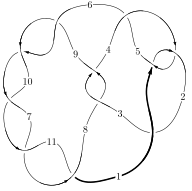
\includegraphics[width=112pt]{../../../GIT/diagram.site/Diagrams/png/311_11a_62.png}\\
\ \ \ A knot diagram\footnotemark}&
\allowdisplaybreaks
\textbf{Linearized knot diagam} \\
\cline{2-2}
 &
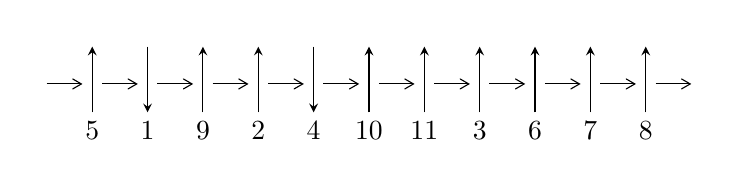
\begin{tikzpicture}[x=20pt, y=17pt]
	% nodes
	\node (C0) at (0, 0) {};
	\node (C1) at (1, 0) {};
	\node (C1U) at (1, +1) {};
	\node (C1D) at (1, -1) {5};

	\node (C2) at (2, 0) {};
	\node (C2U) at (2, +1) {};
	\node (C2D) at (2, -1) {1};

	\node (C3) at (3, 0) {};
	\node (C3U) at (3, +1) {};
	\node (C3D) at (3, -1) {9};

	\node (C4) at (4, 0) {};
	\node (C4U) at (4, +1) {};
	\node (C4D) at (4, -1) {2};

	\node (C5) at (5, 0) {};
	\node (C5U) at (5, +1) {};
	\node (C5D) at (5, -1) {4};

	\node (C6) at (6, 0) {};
	\node (C6U) at (6, +1) {};
	\node (C6D) at (6, -1) {10};

	\node (C7) at (7, 0) {};
	\node (C7U) at (7, +1) {};
	\node (C7D) at (7, -1) {11};

	\node (C8) at (8, 0) {};
	\node (C8U) at (8, +1) {};
	\node (C8D) at (8, -1) {3};

	\node (C9) at (9, 0) {};
	\node (C9U) at (9, +1) {};
	\node (C9D) at (9, -1) {6};

	\node (C10) at (10, 0) {};
	\node (C10U) at (10, +1) {};
	\node (C10D) at (10, -1) {7};

	\node (C11) at (11, 0) {};
	\node (C11U) at (11, +1) {};
	\node (C11D) at (11, -1) {8};
	\node (C12) at (12, 0) {};

	% arrows
	\draw[->,>={angle 60}]
	(C0) edge (C1) (C1) edge (C2) (C2) edge (C3) (C3) edge (C4) (C4) edge (C5) (C5) edge (C6) (C6) edge (C7) (C7) edge (C8) (C8) edge (C9) (C9) edge (C10) (C10) edge (C11) (C11) edge (C12) ;	\draw[->,>=stealth]
	(C1D) edge (C1U) (C2U) edge (C2D) (C3D) edge (C3U) (C4D) edge (C4U) (C5U) edge (C5D) (C6D) edge (C6U) (C7D) edge (C7U) (C8D) edge (C8U) (C9D) edge (C9U) (C10D) edge (C10U) (C11D) edge (C11U) ;
	\end{tikzpicture} \\
\hhline{~~} \\& 
\textbf{Solving Sequence} \\ \cline{2-2} 
 &
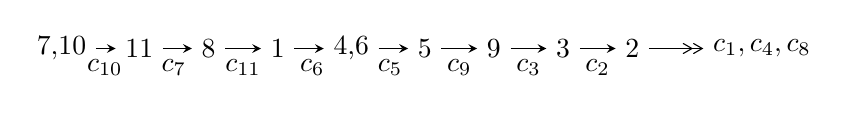
\begin{tikzpicture}[x=25pt, y=7pt]
	% node
	\node (A0) at (-1/8, 0) {7,10};
	\node (A1) at (1, 0) {11};
	\node (A2) at (2, 0) {8};
	\node (A3) at (3, 0) {1};
	\node (A4) at (65/16, 0) {4,6};
	\node (A5) at (41/8, 0) {5};
	\node (A6) at (49/8, 0) {9};
	\node (A7) at (57/8, 0) {3};
	\node (A8) at (65/8, 0) {2};
	\node (C1) at (1/2, -1) {$c_{10}$};
	\node (C2) at (3/2, -1) {$c_{7}$};
	\node (C3) at (5/2, -1) {$c_{11}$};
	\node (C4) at (7/2, -1) {$c_{6}$};
	\node (C5) at (37/8, -1) {$c_{5}$};
	\node (C6) at (45/8, -1) {$c_{9}$};
	\node (C7) at (53/8, -1) {$c_{3}$};
	\node (C8) at (61/8, -1) {$c_{2}$};
	\node (A9) at (10, 0) {$c_{1},c_{4},c_{8}$};

	% edge
	\draw[->,>=stealth]	
	(A0) edge (A1) (A1) edge (A2) (A2) edge (A3) (A3) edge (A4) (A4) edge (A5) (A5) edge (A6) (A6) edge (A7) (A7) edge (A8) ;
	\draw[->>,>={angle 60}]	
	(A8) edge (A9);
\end{tikzpicture} \\ 

\end{tabular} \\

\footnotetext{
The image of knot diagram is generated by the software ``\textbf{Draw programme}" developed by Andrew Bartholomew(\url{http://www.layer8.co.uk/maths/draw/index.htm\#Running-draw}), where we modified some parts for our purpose(\url{https://github.com/CATsTAILs/LinksPainter}).
}\phantom \\ \newline 
\centering \textbf{Ideals for irreducible components\footnotemark of $X_{\text{par}}$} 
 
\begin{align*}
I^u_{1}&=\langle 
3 u^{30}-3 u^{29}+\cdots+2 b-3,\;-5 u^{30}+8 u^{29}+\cdots+2 a+5 u,\;u^{31}-3 u^{30}+\cdots-12 u^2+1\rangle \\
I^u_{2}&=\langle 
- a u+b,\;a^2- a+1,\;u^2+u-1\rangle \\
\\
\end{align*}
\raggedright * 2 irreducible components of $\dim_{\mathbb{C}}=0$, with total 35 representations.\\
\footnotetext{All coefficients of polynomials are rational numbers. But the coefficients are sometimes approximated in decimal forms when there is not enough margin.}
\newpage
\renewcommand{\arraystretch}{1}
\centering \section*{I. $I^u_{1}= \langle 3 u^{30}-3 u^{29}+\cdots+2 b-3,\;-5 u^{30}+8 u^{29}+\cdots+2 a+5 u,\;u^{31}-3 u^{30}+\cdots-12 u^2+1 \rangle$}
\flushleft \textbf{(i) Arc colorings}\\
\begin{tabular}{m{7pt} m{180pt} m{7pt} m{180pt} }
\flushright $a_{7}=$&$\begin{pmatrix}0\\u\end{pmatrix}$ \\
\flushright $a_{10}=$&$\begin{pmatrix}1\\0\end{pmatrix}$ \\
\flushright $a_{11}=$&$\begin{pmatrix}1\\- u^2\end{pmatrix}$ \\
\flushright $a_{8}=$&$\begin{pmatrix}u\\- u^3+u\end{pmatrix}$ \\
\flushright $a_{1}=$&$\begin{pmatrix}- u^2+1\\u^4-2 u^2\end{pmatrix}$ \\
\flushright $a_{4}=$&$\begin{pmatrix}\frac{5}{2} u^{30}-4 u^{29}+\cdots+\frac{11}{2} u^2-\frac{5}{2} u\\-\frac{3}{2} u^{30}+\frac{3}{2} u^{29}+\cdots- u+\frac{3}{2}\end{pmatrix}$ \\
\flushright $a_{6}=$&$\begin{pmatrix}- u\\u\end{pmatrix}$ \\
\flushright $a_{5}=$&$\begin{pmatrix}-\frac{1}{2} u^{30}+u^{29}+\cdots-\frac{11}{2} u+1\\\frac{1}{2} u^{30}-\frac{1}{2} u^{29}+\cdots+\frac{19}{2} u^2-\frac{1}{2}\end{pmatrix}$ \\
\flushright $a_{9}=$&$\begin{pmatrix}- u^2+1\\u^2\end{pmatrix}$ \\
\flushright $a_{3}=$&$\begin{pmatrix}-\frac{9}{2} u^{30}+5 u^{29}+\cdots+\frac{1}{2} u+4\\\frac{17}{2} u^{30}-\frac{21}{2} u^{29}+\cdots-4 u-\frac{9}{2}\end{pmatrix}$ \\
\flushright $a_{2}=$&$\begin{pmatrix}-2 u^{30}+\frac{3}{2} u^{29}+\cdots-\frac{3}{2} u+\frac{7}{2}\\4 u^{30}-5 u^{29}+\cdots-2 u-2\end{pmatrix}$\\ \flushright $a_{2}=$&$\begin{pmatrix}-2 u^{30}+\frac{3}{2} u^{29}+\cdots-\frac{3}{2} u+\frac{7}{2}\\4 u^{30}-5 u^{29}+\cdots-2 u-2\end{pmatrix}$\\&\end{tabular}
\flushleft \textbf{(ii) Obstruction class $= -1$}\\~\\
\flushleft \textbf{(iii) Cusp Shapes $= \frac{13}{2} u^{30}-8 u^{29}+\cdots+\frac{31}{2} u+9$}\\~\\
\newpage\renewcommand{\arraystretch}{1}
\flushleft \textbf{(iv) u-Polynomials at the component}\newline \\
\begin{tabular}{m{50pt}|m{274pt}}
Crossings & \hspace{64pt}u-Polynomials at each crossing \\
\hline $$\begin{aligned}c_{1},c_{4}\end{aligned}$$&$\begin{aligned}
&u^{31}+3 u^{30}+\cdots+4 u-1
\end{aligned}$\\
\hline $$\begin{aligned}c_{2},c_{5}\end{aligned}$$&$\begin{aligned}
&u^{31}+9 u^{30}+\cdots+12 u-1
\end{aligned}$\\
\hline $$\begin{aligned}c_{3},c_{8}\end{aligned}$$&$\begin{aligned}
&u^{31}+u^{30}+\cdots-20 u^2+16
\end{aligned}$\\
\hline $$\begin{aligned}c_{6},c_{7},c_{9}\\c_{10},c_{11}\end{aligned}$$&$\begin{aligned}
&u^{31}-3 u^{30}+\cdots-12 u^2+1
\end{aligned}$\\
\hline
\end{tabular}\\~\\
\newpage\renewcommand{\arraystretch}{1}
\flushleft \textbf{(v) Riley Polynomials at the component}\newline \\
\begin{tabular}{m{50pt}|m{274pt}}
Crossings & \hspace{64pt}Riley Polynomials at each crossing \\
\hline $$\begin{aligned}c_{1},c_{4}\end{aligned}$$&$\begin{aligned}
&y^{31}+9 y^{30}+\cdots+12 y-1
\end{aligned}$\\
\hline $$\begin{aligned}c_{2},c_{5}\end{aligned}$$&$\begin{aligned}
&y^{31}+29 y^{30}+\cdots+524 y-1
\end{aligned}$\\
\hline $$\begin{aligned}c_{3},c_{8}\end{aligned}$$&$\begin{aligned}
&y^{31}-25 y^{30}+\cdots+640 y-256
\end{aligned}$\\
\hline $$\begin{aligned}c_{6},c_{7},c_{9}\\c_{10},c_{11}\end{aligned}$$&$\begin{aligned}
&y^{31}-43 y^{30}+\cdots+24 y-1
\end{aligned}$\\
\hline
\end{tabular}\\~\\
\newpage\flushleft \textbf{(vi) Complex Volumes and Cusp Shapes}
$$\begin{array}{c|c|c}  
\text{Solutions to }I^u_{1}& \I (\text{vol} + \sqrt{-1}CS) & \text{Cusp shape}\\
 \hline 
\begin{aligned}
u &= -0.979024 + 0.144758 I \\
a &= \phantom{-}0.831915 + 0.090072 I \\
b &= \phantom{-}0.119170 + 0.711208 I\end{aligned}
 & \phantom{-}2.01140 - 3.46353 I & \phantom{-}11.93946 + 5.35734 I \\ \hline\begin{aligned}
u &= -0.979024 - 0.144758 I \\
a &= \phantom{-}0.831915 - 0.090072 I \\
b &= \phantom{-}0.119170 - 0.711208 I\end{aligned}
 & \phantom{-}2.01140 + 3.46353 I & \phantom{-}11.93946 - 5.35734 I \\ \hline\begin{aligned}
u &= \phantom{-}1.077390 + 0.054634 I \\
a &= \phantom{-}0.229000 - 1.283970 I \\
b &= -0.36400 + 2.47719 I\end{aligned}
 & \phantom{-}4.65693 + 2.79600 I & \phantom{-}13.44598 - 3.14561 I \\ \hline\begin{aligned}
u &= \phantom{-}1.077390 - 0.054634 I \\
a &= \phantom{-}0.229000 + 1.283970 I \\
b &= -0.36400 - 2.47719 I\end{aligned}
 & \phantom{-}4.65693 - 2.79600 I & \phantom{-}13.44598 + 3.14561 I \\ \hline\begin{aligned}
u &= -1.11047\phantom{ +0.000000I} \\
a &= -1.03356\phantom{ +0.000000I} \\
b &= \phantom{-}0.559359\phantom{ +0.000000I}\end{aligned}
 & \phantom{-}5.42058\phantom{ +0.000000I} & \phantom{-}16.8260\phantom{ +0.000000I} \\ \hline\begin{aligned}
u &= -1.127600 + 0.375707 I \\
a &= \phantom{-}0.299700 - 0.775841 I \\
b &= -0.43314 + 2.13863 I\end{aligned}
 & \phantom{-}9.18803 - 8.59967 I & \phantom{-}14.1525 + 6.5112 I \\ \hline\begin{aligned}
u &= -1.127600 - 0.375707 I \\
a &= \phantom{-}0.299700 + 0.775841 I \\
b &= -0.43314 - 2.13863 I\end{aligned}
 & \phantom{-}9.18803 + 8.59967 I & \phantom{-}14.1525 - 6.5112 I \\ \hline\begin{aligned}
u &= -1.174380 + 0.329803 I \\
a &= -0.642970 + 0.790351 I \\
b &= \phantom{-}0.82679 - 1.90155 I\end{aligned}
 & \phantom{-}9.85498 - 2.40122 I & \phantom{-}15.3857 + 1.4439 I \\ \hline\begin{aligned}
u &= -1.174380 - 0.329803 I \\
a &= -0.642970 - 0.790351 I \\
b &= \phantom{-}0.82679 + 1.90155 I\end{aligned}
 & \phantom{-}9.85498 + 2.40122 I & \phantom{-}15.3857 - 1.4439 I \\ \hline\begin{aligned}
u &= \phantom{-}0.422649 + 0.629353 I \\
a &= -1.064760 - 0.248038 I \\
b &= -0.493860 - 0.673775 I\end{aligned}
 & \phantom{-}4.80361 - 0.89095 I & \phantom{-}12.16176 - 0.45664 I\\
 \hline 
 \end{array}$$\newpage$$\begin{array}{c|c|c}  
\text{Solutions to }I^u_{1}& \I (\text{vol} + \sqrt{-1}CS) & \text{Cusp shape}\\
 \hline 
\begin{aligned}
u &= \phantom{-}0.422649 - 0.629353 I \\
a &= -1.064760 + 0.248038 I \\
b &= -0.493860 + 0.673775 I\end{aligned}
 & \phantom{-}4.80361 + 0.89095 I & \phantom{-}12.16176 + 0.45664 I \\ \hline\begin{aligned}
u &= \phantom{-}0.348369 + 0.655737 I \\
a &= \phantom{-}1.28503 + 0.62780 I \\
b &= \phantom{-}0.291890 + 0.578542 I\end{aligned}
 & \phantom{-}4.57379 + 5.07655 I & \phantom{-}11.28457 - 5.75893 I \\ \hline\begin{aligned}
u &= \phantom{-}0.348369 - 0.655737 I \\
a &= \phantom{-}1.28503 - 0.62780 I \\
b &= \phantom{-}0.291890 - 0.578542 I\end{aligned}
 & \phantom{-}4.57379 - 5.07655 I & \phantom{-}11.28457 + 5.75893 I \\ \hline\begin{aligned}
u &= \phantom{-}0.698660 + 0.209211 I \\
a &= \phantom{-}0.266260 - 0.231304 I \\
b &= -0.762190 + 0.457078 I\end{aligned}
 & \phantom{-}0.456932 + 0.462087 I & \phantom{-}9.00639 - 0.86680 I \\ \hline\begin{aligned}
u &= \phantom{-}0.698660 - 0.209211 I \\
a &= \phantom{-}0.266260 + 0.231304 I \\
b &= -0.762190 - 0.457078 I\end{aligned}
 & \phantom{-}0.456932 - 0.462087 I & \phantom{-}9.00639 + 0.86680 I \\ \hline\begin{aligned}
u &= \phantom{-}0.099887 + 0.392148 I \\
a &= -0.03361 + 1.67355 I \\
b &= \phantom{-}0.443597 + 0.182843 I\end{aligned}
 & -1.25989 + 1.71484 I & \phantom{-}2.62221 - 5.71238 I \\ \hline\begin{aligned}
u &= \phantom{-}0.099887 - 0.392148 I \\
a &= -0.03361 - 1.67355 I \\
b &= \phantom{-}0.443597 - 0.182843 I\end{aligned}
 & -1.25989 - 1.71484 I & \phantom{-}2.62221 + 5.71238 I \\ \hline\begin{aligned}
u &= \phantom{-}0.394527\phantom{ +0.000000I} \\
a &= \phantom{-}0.563421\phantom{ +0.000000I} \\
b &= -0.451465\phantom{ +0.000000I}\end{aligned}
 & \phantom{-}0.662850\phantom{ +0.000000I} & \phantom{-}15.1240\phantom{ +0.000000I} \\ \hline\begin{aligned}
u &= -1.63009 + 0.03537 I \\
a &= -0.815204 - 0.932358 I \\
b &= \phantom{-}1.04001 + 1.19147 I\end{aligned}
 & \phantom{-}8.61876 - 1.24218 I & \phantom{-0.000000 } 0 \\ \hline\begin{aligned}
u &= -1.63009 - 0.03537 I \\
a &= -0.815204 + 0.932358 I \\
b &= \phantom{-}1.04001 - 1.19147 I\end{aligned}
 & \phantom{-}8.61876 + 1.24218 I & \phantom{-0.000000 } 0\\
 \hline 
 \end{array}$$\newpage$$\begin{array}{c|c|c}  
\text{Solutions to }I^u_{1}& \I (\text{vol} + \sqrt{-1}CS) & \text{Cusp shape}\\
 \hline 
\begin{aligned}
u &= -0.268160 + 0.102485 I \\
a &= -0.10435 + 2.92800 I \\
b &= \phantom{-}0.250893 + 0.701619 I\end{aligned}
 & \phantom{-}0.38814 - 2.23506 I & \phantom{-}1.04827 + 4.75217 I \\ \hline\begin{aligned}
u &= -0.268160 - 0.102485 I \\
a &= -0.10435 - 2.92800 I \\
b &= \phantom{-}0.250893 - 0.701619 I\end{aligned}
 & \phantom{-}0.38814 + 2.23506 I & \phantom{-}1.04827 - 4.75217 I \\ \hline\begin{aligned}
u &= \phantom{-}1.72918 + 0.03341 I \\
a &= \phantom{-}0.219808 - 1.029000 I \\
b &= -0.95945 + 1.46832 I\end{aligned}
 & \phantom{-}11.77940 + 4.15554 I & \phantom{-0.000000 } 0 \\ \hline\begin{aligned}
u &= \phantom{-}1.72918 - 0.03341 I \\
a &= \phantom{-}0.219808 + 1.029000 I \\
b &= -0.95945 - 1.46832 I\end{aligned}
 & \phantom{-}11.77940 - 4.15554 I & \phantom{-0.000000 } 0 \\ \hline\begin{aligned}
u &= -1.75006 + 0.01346 I \\
a &= -0.27253 - 3.19299 I \\
b &= \phantom{-}0.33934 + 4.04196 I\end{aligned}
 & \phantom{-}14.9045 - 3.0785 I & \phantom{-0.000000 } 0 \\ \hline\begin{aligned}
u &= -1.75006 - 0.01346 I \\
a &= -0.27253 + 3.19299 I \\
b &= \phantom{-}0.33934 - 4.04196 I\end{aligned}
 & \phantom{-}14.9045 + 3.0785 I & \phantom{-0.000000 } 0 \\ \hline\begin{aligned}
u &= \phantom{-}1.75654\phantom{ +0.000000I} \\
a &= \phantom{-}0.528132\phantom{ +0.000000I} \\
b &= -0.0669841\phantom{ +0.000000I}\end{aligned}
 & \phantom{-}15.8245\phantom{ +0.000000I} & \phantom{-0.000000 } 0 \\ \hline\begin{aligned}
u &= \phantom{-}1.76039 + 0.10095 I \\
a &= -0.77692 - 2.65214 I \\
b &= \phantom{-}0.57757 + 3.62883 I\end{aligned}
 & \phantom{-}19.5055 + 10.6386 I & \phantom{-0.000000 } 0 \\ \hline\begin{aligned}
u &= \phantom{-}1.76039 - 0.10095 I \\
a &= -0.77692 + 2.65214 I \\
b &= \phantom{-}0.57757 - 3.62883 I\end{aligned}
 & \phantom{-}19.5055 - 10.6386 I & \phantom{-0.000000 } 0 \\ \hline\begin{aligned}
u &= \phantom{-}1.77250 + 0.08381 I \\
a &= \phantom{-}1.04963 + 2.23983 I \\
b &= -0.89708 - 3.04423 I\end{aligned}
 & -19.0119 + 4.1870 I & \phantom{-0.000000 } 0\\
 \hline 
 \end{array}$$\newpage$$\begin{array}{c|c|c}  
\text{Solutions to }I^u_{1}& \I (\text{vol} + \sqrt{-1}CS) & \text{Cusp shape}\\
 \hline 
\begin{aligned}
u &= \phantom{-}1.77250 - 0.08381 I \\
a &= \phantom{-}1.04963 - 2.23983 I \\
b &= -0.89708 + 3.04423 I\end{aligned}
 & -19.0119 - 4.1870 I & \phantom{-0.000000 } 0\\
 \hline 
 \end{array}$$\newpage\newpage\renewcommand{\arraystretch}{1}
\centering \section*{II. $I^u_{2}= \langle - a u+b,\;a^2- a+1,\;u^2+u-1 \rangle$}
\flushleft \textbf{(i) Arc colorings}\\
\begin{tabular}{m{7pt} m{180pt} m{7pt} m{180pt} }
\flushright $a_{7}=$&$\begin{pmatrix}0\\u\end{pmatrix}$ \\
\flushright $a_{10}=$&$\begin{pmatrix}1\\0\end{pmatrix}$ \\
\flushright $a_{11}=$&$\begin{pmatrix}1\\u-1\end{pmatrix}$ \\
\flushright $a_{8}=$&$\begin{pmatrix}u\\- u+1\end{pmatrix}$ \\
\flushright $a_{1}=$&$\begin{pmatrix}u\\- u\end{pmatrix}$ \\
\flushright $a_{4}=$&$\begin{pmatrix}a\\a u\end{pmatrix}$ \\
\flushright $a_{6}=$&$\begin{pmatrix}- u\\u\end{pmatrix}$ \\
\flushright $a_{5}=$&$\begin{pmatrix}a- u-1\\a u\end{pmatrix}$ \\
\flushright $a_{9}=$&$\begin{pmatrix}u\\- u+1\end{pmatrix}$ \\
\flushright $a_{3}=$&$\begin{pmatrix}a\\a u\end{pmatrix}$ \\
\flushright $a_{2}=$&$\begin{pmatrix}a u+a\\0\end{pmatrix}$\\ \flushright $a_{2}=$&$\begin{pmatrix}a u+a\\0\end{pmatrix}$\\&\end{tabular}
\flushleft \textbf{(ii) Obstruction class $= 1$}\\~\\
\flushleft \textbf{(iii) Cusp Shapes $= -2 a u+3 a+u+12$}\\~\\
\newpage\renewcommand{\arraystretch}{1}
\flushleft \textbf{(iv) u-Polynomials at the component}\newline \\
\begin{tabular}{m{50pt}|m{274pt}}
Crossings & \hspace{64pt}u-Polynomials at each crossing \\
\hline $$\begin{aligned}c_{1},c_{2},c_{5}\end{aligned}$$&$\begin{aligned}
&(u^2+u+1)^2
\end{aligned}$\\
\hline $$\begin{aligned}c_{3},c_{8}\end{aligned}$$&$\begin{aligned}
&u^4
\end{aligned}$\\
\hline $$\begin{aligned}c_{4}\end{aligned}$$&$\begin{aligned}
&(u^2- u+1)^2
\end{aligned}$\\
\hline $$\begin{aligned}c_{6},c_{7}\end{aligned}$$&$\begin{aligned}
&(u^2- u-1)^2
\end{aligned}$\\
\hline $$\begin{aligned}c_{9},c_{10},c_{11}\end{aligned}$$&$\begin{aligned}
&(u^2+u-1)^2
\end{aligned}$\\
\hline
\end{tabular}\\~\\
\newpage\renewcommand{\arraystretch}{1}
\flushleft \textbf{(v) Riley Polynomials at the component}\newline \\
\begin{tabular}{m{50pt}|m{274pt}}
Crossings & \hspace{64pt}Riley Polynomials at each crossing \\
\hline $$\begin{aligned}c_{1},c_{2},c_{4}\\c_{5}\end{aligned}$$&$\begin{aligned}
&(y^2+y+1)^2
\end{aligned}$\\
\hline $$\begin{aligned}c_{3},c_{8}\end{aligned}$$&$\begin{aligned}
&y^4
\end{aligned}$\\
\hline $$\begin{aligned}c_{6},c_{7},c_{9}\\c_{10},c_{11}\end{aligned}$$&$\begin{aligned}
&(y^2-3 y+1)^2
\end{aligned}$\\
\hline
\end{tabular}\\~\\
\newpage\flushleft \textbf{(vi) Complex Volumes and Cusp Shapes}
$$\begin{array}{c|c|c}  
\text{Solutions to }I^u_{2}& \I (\text{vol} + \sqrt{-1}CS) & \text{Cusp shape}\\
 \hline 
\begin{aligned}
u &= \phantom{-}0.618034\phantom{ +0.000000I} \\
a &= \phantom{-}0.500000 + 0.866025 I \\
b &= \phantom{-}0.309017 + 0.535233 I\end{aligned}
 & \phantom{-}0.98696 - 2.02988 I & \phantom{-}13.50000 + 1.52761 I \\ \hline\begin{aligned}
u &= \phantom{-}0.618034\phantom{ +0.000000I} \\
a &= \phantom{-}0.500000 - 0.866025 I \\
b &= \phantom{-}0.309017 - 0.535233 I\end{aligned}
 & \phantom{-}0.98696 + 2.02988 I & \phantom{-}13.50000 - 1.52761 I \\ \hline\begin{aligned}
u &= -1.61803\phantom{ +0.000000I} \\
a &= \phantom{-}0.500000 + 0.866025 I \\
b &= -0.80902 - 1.40126 I\end{aligned}
 & \phantom{-}8.88264 - 2.02988 I & \phantom{-}13.5000 + 5.4006 I \\ \hline\begin{aligned}
u &= -1.61803\phantom{ +0.000000I} \\
a &= \phantom{-}0.500000 - 0.866025 I \\
b &= -0.80902 + 1.40126 I\end{aligned}
 & \phantom{-}8.88264 + 2.02988 I & \phantom{-}13.5000 - 5.4006 I\\
 \hline 
 \end{array}$$\newpage
\newpage\renewcommand{\arraystretch}{1}
\centering \section*{ III. u-Polynomials}
\begin{tabular}{m{50pt}|m{274pt}}
Crossings & \hspace{64pt}u-Polynomials at each crossing \\
\hline $$\begin{aligned}c_{1}\end{aligned}$$&$\begin{aligned}
&((u^2+u+1)^2)(u^{31}+3 u^{30}+\cdots+4 u-1)
\end{aligned}$\\
\hline $$\begin{aligned}c_{2},c_{5}\end{aligned}$$&$\begin{aligned}
&((u^2+u+1)^2)(u^{31}+9 u^{30}+\cdots+12 u-1)
\end{aligned}$\\
\hline $$\begin{aligned}c_{3},c_{8}\end{aligned}$$&$\begin{aligned}
&u^4(u^{31}+u^{30}+\cdots-20 u^2+16)
\end{aligned}$\\
\hline $$\begin{aligned}c_{4}\end{aligned}$$&$\begin{aligned}
&((u^2- u+1)^2)(u^{31}+3 u^{30}+\cdots+4 u-1)
\end{aligned}$\\
\hline $$\begin{aligned}c_{6},c_{7}\end{aligned}$$&$\begin{aligned}
&((u^2- u-1)^2)(u^{31}-3 u^{30}+\cdots-12 u^2+1)
\end{aligned}$\\
\hline $$\begin{aligned}c_{9},c_{10},c_{11}\end{aligned}$$&$\begin{aligned}
&((u^2+u-1)^2)(u^{31}-3 u^{30}+\cdots-12 u^2+1)
\end{aligned}$\\
\hline
\end{tabular}\newpage\renewcommand{\arraystretch}{1}
\centering \section*{ IV. Riley Polynomials}
\begin{tabular}{m{50pt}|m{274pt}}
Crossings & \hspace{64pt}Riley Polynomials at each crossing \\
\hline $$\begin{aligned}c_{1},c_{4}\end{aligned}$$&$\begin{aligned}
&((y^2+y+1)^2)(y^{31}+9 y^{30}+\cdots+12 y-1)
\end{aligned}$\\
\hline $$\begin{aligned}c_{2},c_{5}\end{aligned}$$&$\begin{aligned}
&((y^2+y+1)^2)(y^{31}+29 y^{30}+\cdots+524 y-1)
\end{aligned}$\\
\hline $$\begin{aligned}c_{3},c_{8}\end{aligned}$$&$\begin{aligned}
&y^4(y^{31}-25 y^{30}+\cdots+640 y-256)
\end{aligned}$\\
\hline $$\begin{aligned}c_{6},c_{7},c_{9}\\c_{10},c_{11}\end{aligned}$$&$\begin{aligned}
&((y^2-3 y+1)^2)(y^{31}-43 y^{30}+\cdots+24 y-1)
\end{aligned}$\\
\hline
\end{tabular}
\vskip 2pc
\end{document}